\documentclass[aspectratio=169,11pt]{beamer}
\usetheme{Boadilla}
\usecolortheme{seahorse}
\usepackage[T1]{fontenc}
\usepackage[utf8]{inputenc}
\usepackage{lmodern}
\usepackage{booktabs}
\usepackage{amsmath}
\usepackage{graphicx}
\usepackage{hyperref}
\setbeamertemplate{navigation symbols}{}
\setbeamertemplate{footline}[frame number]
\setbeamerfont{frametitle}{series=\bfseries}

\title{Predicting while optimizing}
\subtitle{Mobile clinic routing with learned constraints}
\author{Joaquim Gromicho \\[1mm] {\small joint work with Mayukh Ghosh and Chintan Amrit}}
\institute{Amsterdam Business School, University of Amsterdam}
\date{Chapter 6 of Mayukh Ghosh's PhD thesis, \emph{Domain Driven Analytics}}

\begin{document}

\begin{frame}
  \titlepage
\end{frame}

% ---------------------------------------------------------------- hook
\begin{frame}{Same history, same solver, same number of stops}
  \centering
  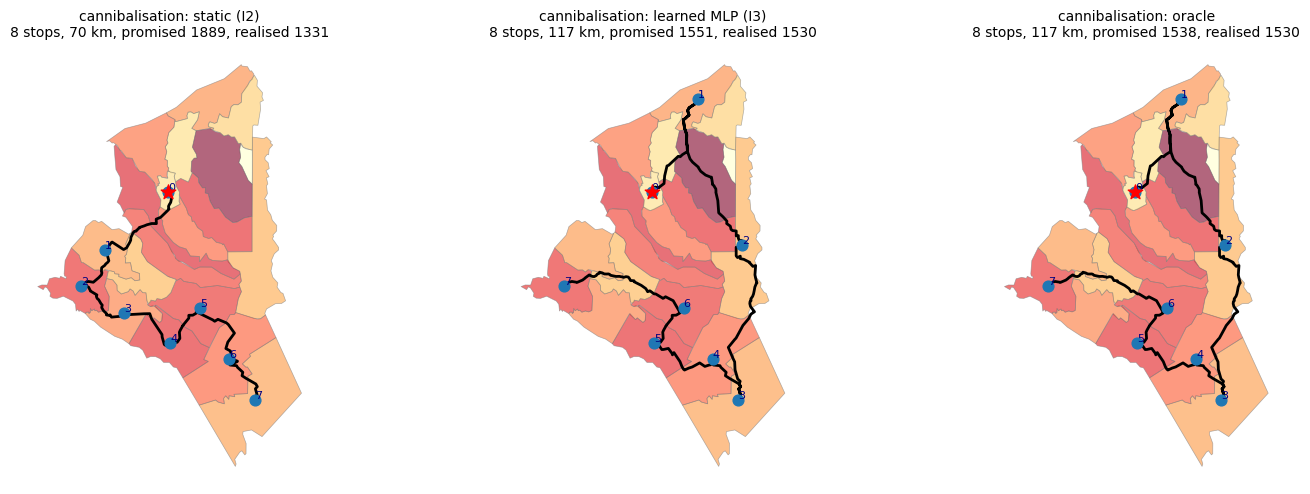
\includegraphics[width=\textwidth]{figs/routes_top.png}
  \vspace{2mm}
  \begin{block}{}
    \centering Left: 1889 doses promised, 1331 delivered. \quad Middle: 1551 promised, 1530 delivered. \quad Why?
  \end{block}
\end{frame}

% ---------------------------------------------------------------- setting
\begin{frame}{The setting: one mobile clinic, many wards}
  \begin{columns}[T]
    \begin{column}{0.55\textwidth}
      \begin{itemize}
        \item AMREF Health Africa ran mobile clinics for COVID-19 vaccination in Kenya (Ghosh, Amrit, Gromicho; thesis Chapter 6).
        \item One clinic, a planning period of a few weeks, at most a handful of stops.
        \item Vaccines are collected at a referral hospital, so the route is an open path from town.
        \item Which wards to visit, and in what order?
      \end{itemize}
      \vspace{2mm}
      Today: Nyamira County, 20 wards, 745 thousand people, 897 km$^2$.
    \end{column}
    \begin{column}{0.45\textwidth}
      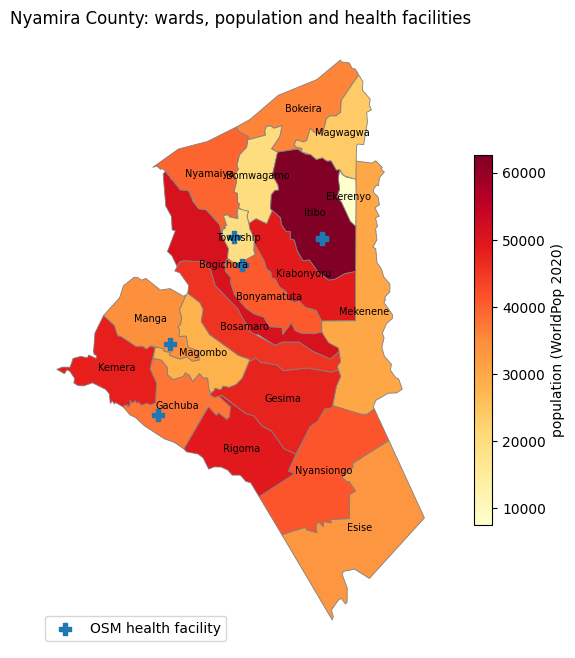
\includegraphics[width=\textwidth,height=0.72\textheight,keepaspectratio]{figs/map.png}
    \end{column}
  \end{columns}
\end{frame}

% ---------------------------------------------------------------- pipeline
\begin{frame}{Predict-then-optimize, and its hidden assumption}
  \begin{enumerate}
    \item Predict demand $\hat d_i$ per ward from population, unvaccinated share, accessibility.
    \item Solve a prize-collecting routing problem that rewards $\hat d_i$ at visited wards.
  \end{enumerate}
  \vspace{3mm}
  \begin{alertblock}{Hidden assumption}
    Demand at ward $i$ does not depend on which other wards the clinic visits.
  \end{alertblock}
  \vspace{3mm}
  Two reasons it does:
  \begin{itemize}
    \item \textbf{Cannibalisation}: people near a visited ward get their dose there; a later visit next door finds less demand.
    \item \textbf{Mobilisation}: health volunteers, market days and word of mouth raise turnout around a visited ward.
  \end{itemize}
\end{frame}

% ---------------------------------------------------------------- spillover
\begin{frame}{Spillover in one formula}
  Let $y_j = 1$ if the clinic visits ward $j$, and $d_{ij}$ the road distance.
  \[
    E_i(y) = \min\Bigl(1,\ \sum_{j \neq i} e^{-d_{ij}/R}\, y_j\Bigr)
    \qquad\qquad
    D_i(y) = b_i \bigl(1 + \gamma\, E_i(y)\bigr)\, \varepsilon_i
  \]
  \begin{itemize}
    \item $E_i$: exposure of ward $i$ to visits nearby, range $R$ (10 km today); one adjacent visit gives about 0.6, two saturate it.
    \item $b_i$: base demand if visited alone; grows with population, unvaccinated share, distance to the nearest facility.
    \item $\gamma < 0$ cannibalisation, $\gamma > 0$ mobilisation, $\gamma = 0$ the textbook case.
    \item The clinic administers at most 250 doses per visit.
  \end{itemize}
  \vspace{2mm}
  Real turnout data would replace the simulator; the structure of the question stays.
\end{frame}

% ---------------------------------------------------------------- data
\begin{frame}{Open data, no API keys}
  \begin{center}
    \begin{tabular}{ll}
      \toprule
      Ingredient & Source \\
      \midrule
      Ward boundaries & GADM 4.1, level 3 \\
      Population per ward & WorldPop 2020, 1 km, UN-adjusted \\
      Road network, health facilities & OpenStreetMap through \texttt{osmnx} \\
      Road distances between wards & \texttt{pandana} contraction hierarchies, 20 by 20 in milliseconds \\
      Demand & simulator above, both signs of $\gamma$ \\
      Optimization & Gurobi, under the free Community Edition limit \\
      \bottomrule
    \end{tabular}
  \end{center}
  \vspace{2mm}
  Caveat: OpenStreetMap lists only 6 health facilities in Nyamira; the Kenya Master Health Facility Registry lists far more.
\end{frame}

% ---------------------------------------------------------------- learning
\begin{frame}{Learning a demand model that contains the decision}
  Where does a training set with $y$ in it come from? Replay the history of past deployments.
  \vspace{2mm}
  \begin{center}
    \begin{tabular}{lcccc|c}
      \toprule
      period, ward & $\log$ pop & unvaccinated & inaccessibility & exposure $E_i$ & turnout $D_i$ \\
      \midrule
      1, Esise   & 10.4 & 0.41 & 1.00 & 0.31 & 361 \\
      1, Gesima  & 10.8 & 0.52 & 0.49 & 1.12 & 275 \\
      2, Gesima  & 10.8 & 0.52 & 0.49 & 0.08 & 560 \\
      $\vdots$ & & & & & \\
      \bottomrule
    \end{tabular}
  \end{center}
  \vspace{2mm}
  \begin{itemize}
    \item 1500 random deployments of 3 to 10 wards, 30\,000 rows.
    \item Two models: linear regression (transparent, mis-specified) and an 8-unit ReLU network, fitted with L-BFGS in seconds.
    \item In practice: past periods' routes plus ticketed turnout, the feedback loop AMREF asked for.
  \end{itemize}
\end{frame}

% ---------------------------------------------------------------- formulation
\begin{frame}{The routing model}
  \small
  Wards $N$, depot $s$, arcs $A$, road distance $c_{ij}$, cost $\mu$ per km, stop limit $K$, capacity $C$ per visit, spillover weights $w_{ij}$, ward features $f_i$, $M = 4C$.
  $x_{ij}, y_i \in \{0,1\}$: drive $i \to j$, visit $i$; $E_i \in [0,1]$ exposure; $\hat d_i \ge 0$ modelled demand; $z_i \in [0, C]$ doses delivered.
  \[
  \begin{array}{rrcll}
  \max & \sum_{i \in N} z_i - \mu \sum_{(i,j) \in A} c_{ij} x_{ij} \\[1mm]
  \text{s.t.} & y_s = 1,\ \sum_j x_{sj} = 1,\ \sum_j x_{js} & = & 0 & \text{path starts at the depot} \\
  & \sum_{j \neq i} x_{ji} & = & y_i & \forall i \neq s \\
  & \sum_{j \neq i} x_{ij} & \le & y_i & \forall i \in N \\
  & \sum_{(i,j) \in A} x_{ij} & = & \sum_{i} y_i - 1, \qquad \sum_i y_i \le K \\
  & E_i & = & \min\bigl(1, \sum_{j \neq i} w_{ij} y_j\bigr) & \forall i \in N \\
  & \hat d_i & \le & g(f_i, E_i) + M(1 - y_i) & \forall i \in N \quad \text{the demand model} \\
  & z_i & \le & \hat d_i, \quad z_i \le C y_i & \forall i \in N \\
  & \sum_{i,j \in S} x_{ij} & \le & \sum_{i \in S} y_i - y_k & \forall S \subseteq N \setminus \{s\},\ k \in S \quad \text{DFJ, lazy}
  \end{array}
  \]
  The DFJ family is generated in a \texttt{MIPSOL} callback with \texttt{cbLazy}: follow the successors from the depot, every visited ward not reached lies on a cycle $S$. Details and the MTZ comparison: MO-book, \href{https://mobook.github.io/MO-book/notebooks/04/08-traveling-salesman-problem.html}{Traveling Salesman Problem}.
\end{frame}

% ---------------------------------------------------------------- model
\begin{frame}{Three ways to fill in $g$ inside the same routing model}
  Same path constraints, same objective; only the demand model $g$ changes.
  \vspace{2mm}
  \begin{center}
    \begin{tabular}{lll}
      \toprule
      Variant & Thesis analogue & The demand model $g$ \\
      \midrule
      static  & Intervention I2 & $g(f_i,\, 0)$, a number fixed before solving \\
      learned & Intervention I3 & $g(f_i,\, E_i)$, the fitted model embedded as constraints \\
      oracle  & upper bound     & $b_i\,(1 + \gamma E_i)$, the simulator's own mean \\
      \bottomrule
    \end{tabular}
  \end{center}
  \vspace{2mm}
  \begin{itemize}
    \item Embedding: one call, \texttt{add\_predictor\_constr(model, g, features, output)} from \texttt{gurobi-machinelearning}.
    \item Size with the network: 980 variables, 404 constraints, no subtour constraint among them. Solves in about a second.
    \item The oracle is linear in $y$ once $E_i$ is in the model, so it is an exact MIP, not a simulation.
  \end{itemize}
\end{frame}

% ---------------------------------------------------------------- results 1
\begin{frame}{Promised versus delivered}
  \centering
  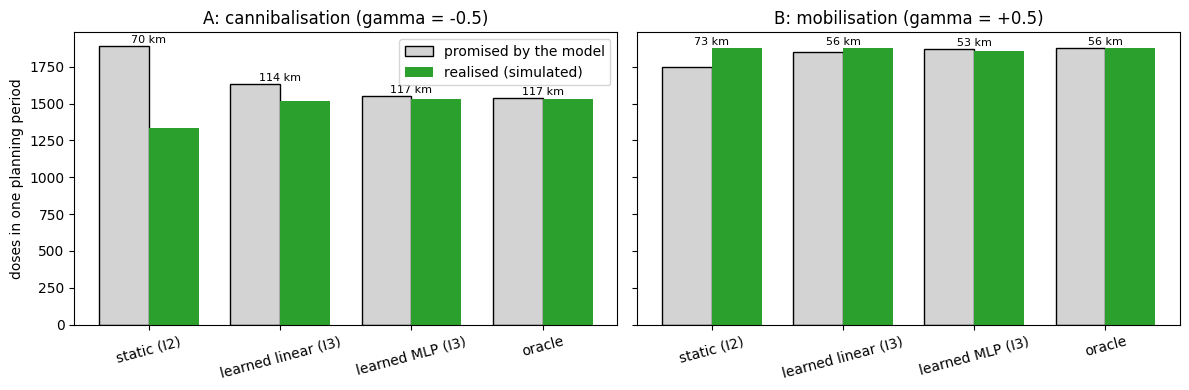
\includegraphics[width=0.95\textwidth]{figs/bars.png}
  \vspace{1mm}
  \begin{itemize}
    \item Cannibalisation: the static plan delivers 70\% of what it promises; the learned network delivers 99\% and 15\% more doses.
    \item Mobilisation: the same doses, but the static plan drives 73 km where 53 km suffice; doses per km go from 26 to 35.
    \item The realised-to-promised ratio is a diagnostic any programme can compute after the fact.
  \end{itemize}
\end{frame}

% ---------------------------------------------------------------- results 2
\begin{frame}{The two signs pull the route in opposite directions}
  \centering
  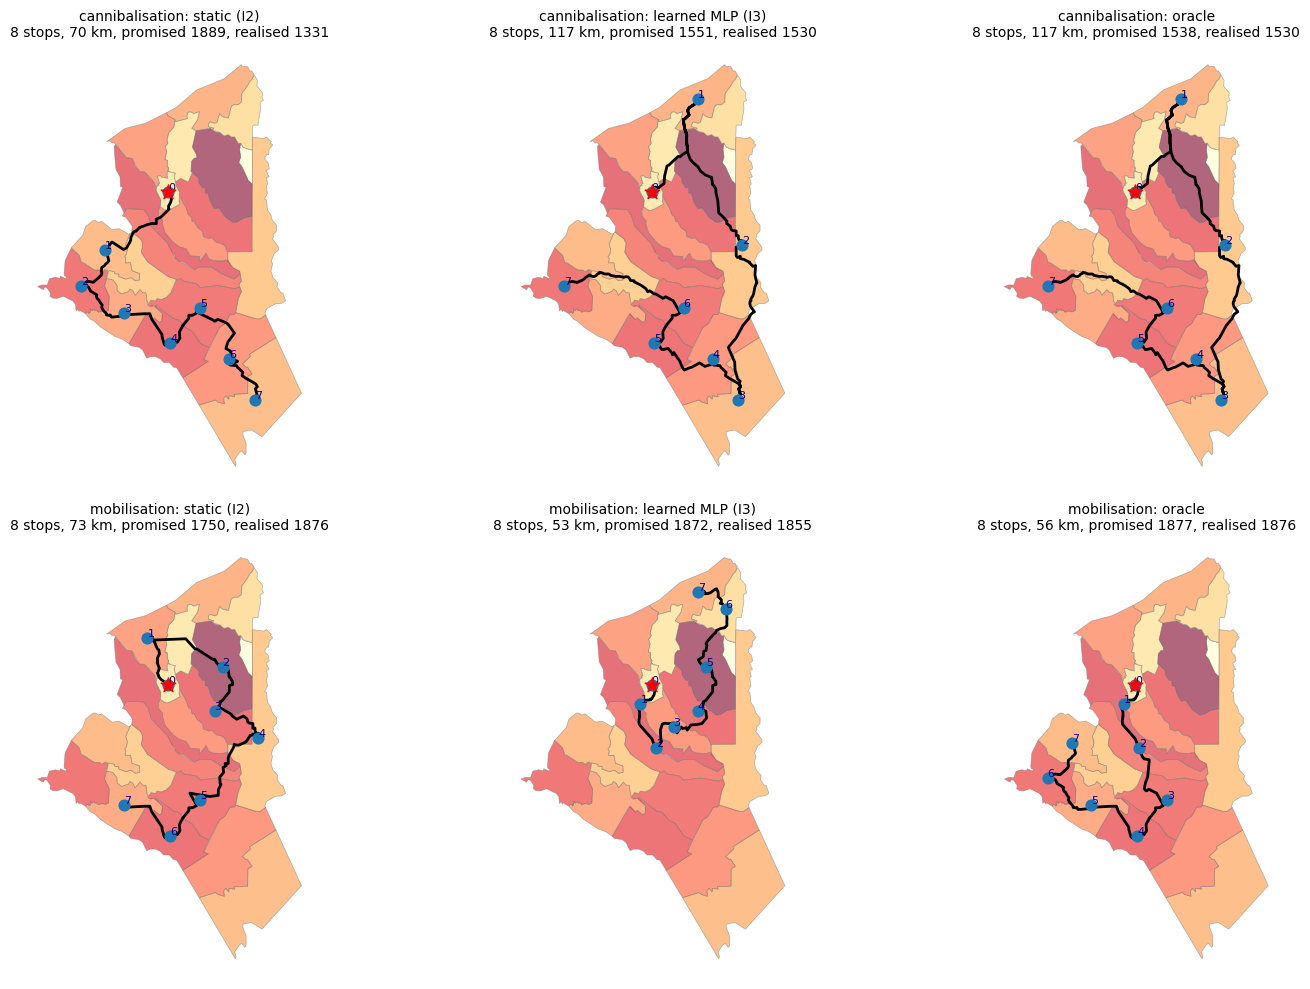
\includegraphics[height=0.82\textheight,keepaspectratio]{figs/routes.png}
\end{frame}

% ---------------------------------------------------------------- sweep
\begin{frame}{How much does it matter? Sweep the interaction strength}
  \begin{columns}[T]
    \begin{column}{0.68\textwidth}
      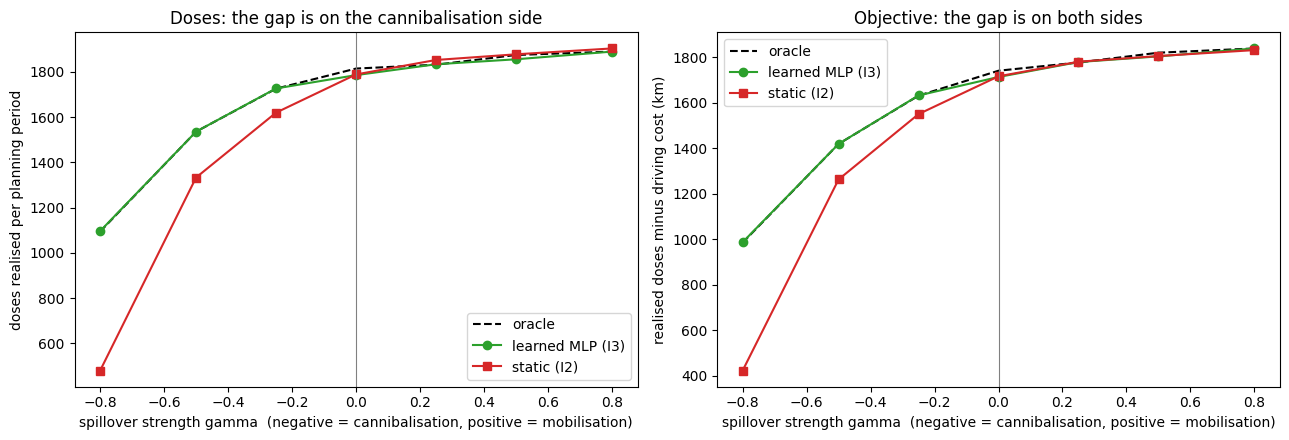
\includegraphics[width=\textwidth]{figs/sweep.png}
    \end{column}
    \begin{column}{0.32\textwidth}
      \vspace{4mm}
      \begin{itemize}
        \item At $\gamma = 0$ the three coincide, as they should.
        \item Cannibalisation costs doses; mobilisation costs kilometres. Only the objective panel shows both.
        \item Models are retrained per $\gamma$; the learned line tracks the oracle throughout.
      \end{itemize}
    \end{column}
  \end{columns}
\end{frame}

% ---------------------------------------------------------------- hands-on
\begin{frame}{Hands-on: ten minutes, one experiment each}
  Open the notebook (link on the board). Outputs are already there; change one parameter, rerun the scenario cell.
  \vspace{2mm}
  \begin{enumerate}
    \item \textbf{Range.} Set \texttt{R\_KM} to 5, then 20. Does the gap between static and learned grow or shrink? Why?
    \item \textbf{Stops.} Set \texttt{K\_STOPS} to 4, then 12. At which end can the static planner ignore spillover?
    \item \textbf{Model size.} Set \texttt{hidden\_layer\_sizes} to \texttt{(2,)}. Watch the variable count and the realised doses. What did you trade?
  \end{enumerate}
  \vspace{3mm}
  Each rerun takes under a minute: data is cached, every solve is about a second.
\end{frame}

% ---------------------------------------------------------------- debrief
\begin{frame}{Debrief and the open question}
  \begin{itemize}
    \item The planner's error is structural, not statistical: both planners saw the same data.
    \item Predicting while optimizing means the prediction is a constraint, not an input.
    \item Keep the model small enough to embed: a linear or tree model, or a one-layer network.
  \end{itemize}
  \vspace{4mm}
  \begin{block}{Open question for research and for practice}
    In a real deployment, where does the training data with decisions in it come from, and how many periods are needed before the learned constraints beat a careful static forecast?
  \end{block}
  \vspace{4mm}
  \small Notebook and code: \texttt{mobile\_clinic\_routing.ipynb}. Thesis: M.\ Ghosh, \emph{Domain Driven Analytics}, University of Amsterdam, Chapter 6.
\end{frame}

\end{document}
